\documentclass[10pt]{article}
\usepackage{fullpage}
\usepackage{graphicx}
\usepackage{url}
\usepackage{hyperref}
\usepackage{rotating}
\usepackage{caption}
\usepackage{color}
\usepackage{fancybox}
\usepackage{fancyvrb}
\usepackage[T1]{fontenc}

%opening
\title{CMSC 23300 -- Networks and Distributed Systems\\{\large Project 2: Transmission Control Protocol}}
\date{}

\newcommand{\chitcp}{$\chi$\textsf{TCP} }
\newcommand{\chisocket}{$\chi$\textsf{socket} }

\newcommand{\RFC}[1]{\href{http://tools.ietf.org/html/rfc#1}{[RFC#1]}}
\newcommand{\RFCsection}[2]{\href{http://tools.ietf.org/html/rfc#1\#section-#2}{[RFC#1 \textsection #2]}}

\newcommand{\points}[1]{{\sffamily\mdseries\guillemotleft #1 points\guillemotright{}}}

\definecolor{backgroundgray}{gray}{0.9}

\fvset{tabsize=2}
\DefineVerbatimEnvironment{VerbExample}{BVerbatim}{boxwidth=0.9\textwidth,fontsize=\footnotesize,samepage=true,commandchars=\\\{\}}
\newenvironment{example}%
{\VerbatimEnvironment\begin{Sbox}\begin{VerbExample}}%
{\end{VerbExample}\end{Sbox}\setlength{\fboxsep}{8pt}\begin{center}\fcolorbox{black}{backgroundgray}{\TheSbox}\end{center}}

\begin{document}
\pagestyle{empty}
\maketitle

\section{Introduction}

In this project you will be implementing the Transmission Control Protocol, as specified in \RFC{793}. However, instead of implementing it inside the operating system itself, you will be implementing it inside a system called \chitcp. This system allows you to write socket-based applications that rely on your TCP implementation instead of the one included in your operating system. To do this, \chitcp provides an alternate socket library, \chisocket, that provides the same functions as the standard socket library (\texttt{connect}, \texttt{send}, \texttt{recv}, etc.). Although the \chisocket functions have the same expected behaviour as the standard socket functions, they do not implement the entire functionality provided by standard sockets (e.g., non-blocking sockets are not supported).

In \chitcp, the socket layer and all the messy details of how TCP interacts with the other layers of the protocol stack (including how packets are handed down to the network layer, and how data is passed up to the application layer) are already implemented for you. In this project, you will focus on implementing the TCP protocol itself.



\section{The \chitcp architecture}
\label{sec:arch}

When using \chitcp in place of the operating system's TCP/IP stack, applications use \chisocket functions to perform standard socket operations, like connect, send, recv, etc. Instead of including the \texttt{socket.h} system header, a \chitcp header must be included:

\begin{example}
#include "chitcp/socket.h"
\end{example}

The functions provided by the \chisocket library are the same as the ones in the standard socket library, except they are prefixed with \texttt{chisocket\_}. They provide essentially the same functionality, although they do not support every possible flag and error code. However, this is enough to write simple clients and servers. For example:

\begin{example}
clientSocket = chisocket_socket(PF_INET,       // Family: IPv4
                                SOCK_STREAM,   // Type: Full-duplex stream (reliable)
                                IPPROTO_TCP);  // Protocol: TCP;

chitcp_addr_construct(host, port, &serverAddr);

chisocket_connect(clientSocket, (struct sockaddr *) &serverAddr, sizeof(struct sockaddr_in));

chisocket_send(clientSocket, "Hello!", 6, 0);

chisocket_close(clientSocket);
\end{example}

For a host to be able to use \chitcp or, more specifically, to be able to write servers and clients based on the \chisocket library instead of the regular socket library, that host must run a \chitcp daemon (called \texttt{chitcpd}). This daemon is where your implementation of TCP will reside, with the \chisocket library performing the standard socket operations (connect, send, recv, etc.) through the \chitcp daemon, instead of accessing the operating system's TCP/IP stack directly.

\begin{figure}
\begin{center}
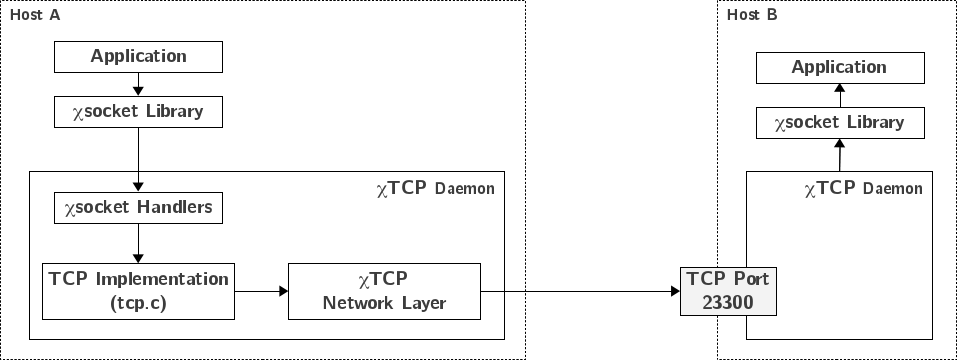
\includegraphics[width=1\textwidth]{architecture.png}
\caption{The \chitcp architecture}
\label{fig:architecture}
\end{center}
\end{figure}

Figure~\ref{fig:architecture} summarizes the \chitcp architecture. Applications that want to use \chitcp call the socket functions in the \chisocket library, which communicates with the \chitcp daemon. This daemon includes three important components:

\begin{itemize}
 \item The \chisocket Handlers: This contains the implementation of the socket layer, and is the interface between an application and your TCP implementation.
 \item The TCP Implementation (file \texttt{tcp.c}, described in more detail in Section~\ref{sec:tcpc}): Your TCP implementation.
 \item The \chitcp Network Layer: This part of the daemon is responsible for getting your TCP packet from one \chitcp daemon to another, the same way that, when using your operating system's TCP/IP stack, IP is responsible for getting your TCP packet from your host to another host.
\end{itemize}

The \chitcp Network Layer is actually just regular TCP (i.e., the operating system's TCP, \emph{not} the one you are implementing). So, when \chitcp needs to get one of your TCP packets to another host, it does so by establishing a (real) TCP connection to that other host's \chitcp daemon on port 23300. Figure~\ref{fig:layers} shows the packet encapsulation that happens in \chitcp. Notice how, from \chitcp's perspective, (real) TCP is essentially the \emph{Network} layer of the protocol stack, while your implementation of TCP is the \emph{Transport} layer. If we looked at this from a standard TCP/IP perspective, your TCP would simply be the payload of a (real) TCP packet.


\begin{sidewaysfigure}
\begin{center}
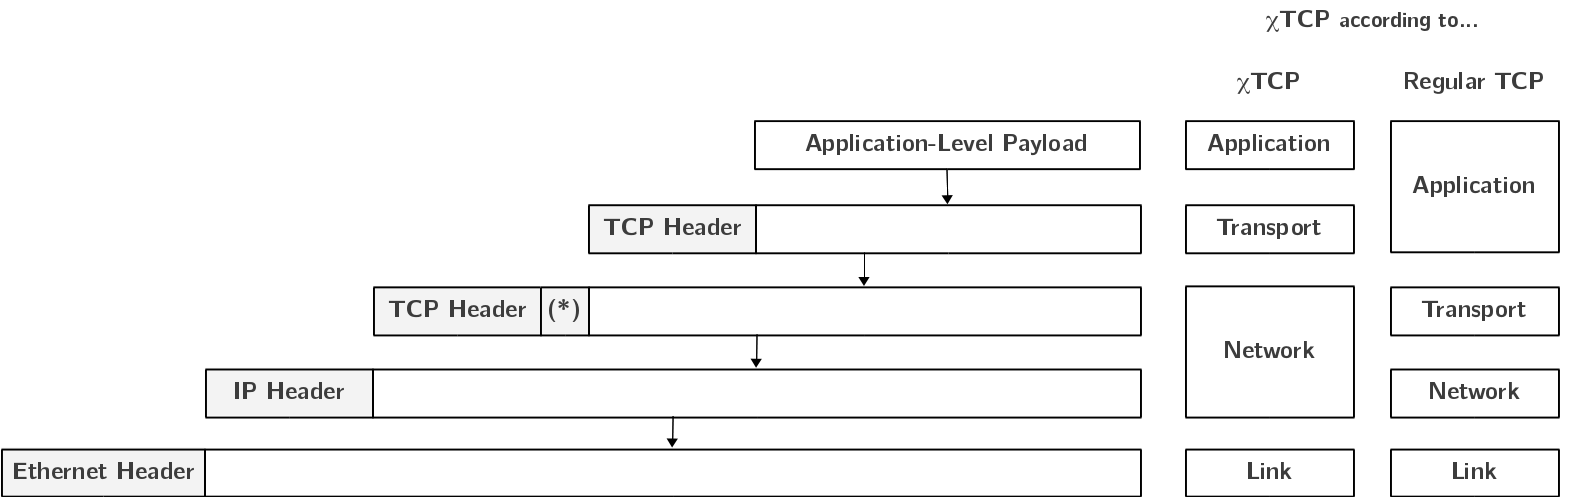
\includegraphics[width=1\textheight]{layers.png}
\caption{The \chitcp layers.\\ \textsf{(*)} \chitcp inserts a special header between the two TCP headers that contains \chitcp-specific information.}
\label{fig:layers}
\end{center}
\end{sidewaysfigure}

\section{Implementing RFC 793}

In this project, you are going to implement a substantial portion of \RFC{793}. In particular, you will be focusing on \RFCsection{793}{3.9} (Event Processing), which provides a detailed description of how TCP should behave (whereas the preceding sections focus more on describing use cases, header specifications, example communications, etc.). The second paragraph of this section sums up pretty nicely how a TCP implementation should behave:

\begin{example}
  The activity of the TCP can be characterized as responding to events.
  The events that occur can be cast into three categories:  user calls,
  arriving segments, and timeouts.  This section describes the
  processing the TCP does in response to each of the events.  In many
  cases the processing required depends on the state of the connection.
\end{example}

So, we can think of TCP as a state machine where:

\begin{itemize}
 \item The states are CLOSED, LISTEN, SYN\_SENT, etc.
 \item The inputs are a series of events defined in \RFC{793} (described below)
 \item The transition from one TCP state to another is based on the current state, an event, \emph{and} a series of TCP variables (SND.NXT, SND.UNA, etc.)
 \item Transitions from one TCP state to another result in actions, typically sending a TCP packet with information dependent on the state of the TCP variables and the send/receive buffers.
\end{itemize}

The events defined in \RFCsection{793}{3.9} are:

\begin{itemize}
 \item \texttt{OPEN}: \chitcp will generate this event when the application layer calls \texttt{chisocket\_connect}.
 \item \texttt{SEND}: \chitcp will generate this event when the application layer calls \texttt{chisocket\_send}.
 \item \texttt{RECEIVE}: \chitcp will generate this event when the application layer calls \texttt{chisocket\_recv}.
 \item \texttt{CLOSE}: \chitcp will generate this event when the application layer calls \texttt{chisocket\_close}.
 \item \texttt{ABORT}: Not supported by \chitcp.
 \item \texttt{STATUS}: Not supported by \chitcp.
 \item \texttt{SEGMENT ARRIVES}: \chitcp will generate this event when a TCP packet arrives.
 \item \texttt{USER TIMEOUT}: Not supported by \chitcp.
 \item \texttt{RETRANSMISSION TIMEOUT}: Not supported by \chitcp.
 \item \texttt{TIME-WAIT TIMEOUT}: Not supported by \chitcp.
\end{itemize}

As described in the next section, your work in \chitcp will center mostly on a file called \texttt{tcp.c} where you are provided with functions that handle events in given TCP states. These functions are initially mostly empty, and it is up to you to write the code that will handle each event in each state.

Of course, a TCP implementation would have to consider every possible combination of states and events. However, many of these are actually invalid combinations. For example, \RFCsection{793}{3.9} specifies that that if the \texttt{SEND} event happens in the following states:

\begin{example}
    FIN-WAIT-1 STATE
    FIN-WAIT-2 STATE
    CLOSING STATE
    LAST-ACK STATE
    TIME-WAIT STATE
\end{example}

Then the following action must be taken:

\begin{example}
      Return "error:  connection closing" and do not service request.
\end{example}

Actions like this are actually handled in the \chisocket layer, and you will not have to worry about them. For example, in the above case, the \texttt{chisocket\_send} function will set \texttt{errno} to \texttt{ENOTCONN}.

Sections \ref{sec:proj2a} and \ref{sec:proj2b} carve out exactly what state/event combinations you will have to implement. Additionally, your implementation should take the following into account:

\begin{itemize}
 \item You can assume a reliable network. You do not need to implement retransmissions or timeouts.
 \item You do not need to support delayed acknowledgements. An acknowledgement packet is sent immediately when data is received, although you can piggyback any data in the send buffer that is waiting to be sent (but you do not need to wait for a timeout to increase the probability that you'll be able to piggyback data on the acknowledgement).
 \item You do not need to support the \texttt{RST} bit.
 \item You do not need to support the \texttt{PSH} bit.
 \item You do not need to support the Urgent Pointer field or the \texttt{URG} bit in the TCP header. This also means you do not need to support the \texttt{SND.UP}, \texttt{RCV.UP}, or \texttt{SEG.UP} variables.
 \item You do not need to support TCP's ``security/compartment'' features, which means you can assume that \texttt{SEG.PRC} and \texttt{TCB.PRC} always have valid and correct values.
 \item You do not need to support the checksum field of the TCP header.
 \item You do not need to support TCP options.
 \item You do not need to support the \texttt{TIME\_WAIT} timeout. You should still update the TCP state to \texttt{TIME\_WAIT} when required, but do not have to implement a timeout. Instead, you should immediately transition to \texttt{CLOSED} from the \texttt{TIME\_WAIT} state.
 \item You do not need to support simultaneous opens (i.e., the transition from \texttt{SYN\_SENT} to \texttt{SYN\_RCVD}).
\end{itemize}



\section{Implementing the \texttt{tcp.c} file}
\label{sec:tcpc}

Since TCP is essentially a state machine, \chitcp's implementation boils down to having a handler function for each of the TCP states (CLOSED, LISTEN, SYN\_RCVD, etc.), all contained in the \texttt{src/chitcpd/tcp.c} file. If an event happens (e.g., a packet arrives) while the connection is in a specific state (e.g., ESTABLISHED), then the handler function for that state is called, along with information about the event that just happened. You will only have to worry about writing the code inside the handler function; the rest of the scaffolding (the socket library, the actual dispatching of events to the state machine, etc.) is already provided for you.
 
Each handler function has the following prototype:
 
\begin{example}
int chitcpd_tcp_state_handle_STATENAME(serverinfo_t *si, 
                                       chisocketentry_t *entry, 
                                       tcp_event_type_t event);
\end{example}

The parameters to the function are:

\begin{itemize}
 \item \texttt{si} is a pointer to a struct with the \chitcp daemon's runtime information (e.g., the socket table, etc.). You should not need to access or modify any of the data in that struct, but you will need the \texttt{si} pointer to call certain auxiliary functions.
 \item \texttt{entry} is a pointer to the socket entry for the connection that is being handled. The socket entry contains the actual TCP data (variables, buffers, etc.), which can be accessed like this:
 
 \begin{example}
 tcp_data_t *tcp_data = &entry->socket_state.active.tcp_data;
 \end{example}
 
The contents of the \texttt{tcp\_data\_t} struct are described below. You should not access or modify any other information in \texttt{entry}.
\item \texttt{event} is the event that is being handled. The list of possible events corresponds roughly to the ones specified in \RFCsection{793}{3.9}. They are:

\begin{itemize}
\item \texttt{APPLICATION\_CONNECT}: Application has called \texttt{chisocket\_connect()} and a three-way handshake must be initiated.
\item \texttt{APPLICATION\_SEND}: Application has called \texttt{chisocket\_send()}. The socket layer (which is already implemented for you) already takes care of placing the data in the socket's TCP send buffer. This event is a notification that there may be new data in the send buffer, which should be sent if possible.
\item \texttt{APPLICATION\_RECEIVE}: Application has called \texttt{chisocket\_recv()}. The socket layer already takes care of extracting the data from the socket's TCP receive buffer. This event is a notification that there may now be additional space available in the receive buffer, which would require updating the socket's receive window (and the advertised window).
\item \texttt{APPLICATION\_CLOSE}: Application has called \texttt{chisocket\_close()} and a connection tear-down should be initiated once all outstanding data in the send buffer has been sent.
\item \texttt{PACKET\_ARRIVAL}: A packet has arrived through the network and needs to be processed (RFC 793 calls this "SEGMENT ARRIVES")
\item \texttt{TIMEOUT}\footnote{Not currently supported in \chitcp}: A timeout (e.g., a retransmission timeout) has happened.
\end{itemize}
\end{itemize}

To implement the TCP protocol, you will need to implement the handler functions in \texttt{tcp.c}. You should not need to modify any other file. However, you will need to use a number of functions and structs defined elsewhere.

\subsection{The \texttt{tcp\_data\_t} struct}

This struct contains all the TCP data for a given socket:

\begin{description}
 \item[The pending packet queue]

\begin{example}
list_t pending_packets;
pthread_mutex_t lock_pending_packets;
pthread_cond_t cv_pending_packets;
\end{example}

As TCP packets arrive through the network, the \chitcp daemon places them in the pending packet queue of the appropriate socket (you do not need inspect the origin and destination port of the TCP packet; this is taken care of for you). The list contains pointers to \texttt{tcp\_packet\_t} structs (described below) in the heap. It is your responsibility to free this memory when you are done processing a packet.

The queue is implemented with the SimCList library, which is already included in the \chitcp code, and the head of the queue can be retrieved using SimCList's \texttt{list\_fetch} function. The \texttt{lock\_pending\_packets} mutex provides thread-safe access to the queue. The \texttt{cv\_pending\_packets} condition variable is used to notify other parts of the \chitcp code that there are new packets in the queue; you should not wait or signal this condition variable.


\item[The TCP variables]

\begin{example}
/* Send sequence variables */
uint32_t ISS;      /* Initial send sequence number */
uint32_t SND_UNA;  /* First byte sent but not acknowledged */
uint32_t SND_NXT;  /* Next sendable byte */
uint32_t SND_WND;  /* Send Window */

/* Receive sequence variables */
uint32_t IRS;      /* Initial receive sequence number */
uint32_t RCV_NXT;  /* Next byte expected */
uint32_t RCV_WND;  /* Receive Window */
\end{example}

These are the TCP sequence variables as specified in \RFCsection{793}{3.2}.

\item[The TCP buffers]

\begin{example}
circular_buffer_t send;
circular_buffer_t recv;
\end{example}

These are the TCP send and receive buffers for this socket. The \texttt{circular\_buffer\_t} type is defined in the \texttt{include/chitcp/buffer.h} and \texttt{src/libchitcp/buffer.c} files. You are provided with a rudimentary (and not actually circular) implementation of this type, which will be enough to run some basic tests with your TCP implementation. However, part of this assignment will involve implementing a better buffer (see Project 2a below).

The management of these buffers is already partially implemented:

\begin{itemize}
 \item The \texttt{chisocket\_send()} function places data in the send buffer and generates an \texttt{APPLICATION\_SEND} event.
 \item The \texttt{chisocket\_recv()} function extracts data from the receive buffer and generates an \texttt{APPLICATION\_RECV} event.
\end{itemize}

In other words, you do not need to implement the above functionality; it is already implemented for you. On the other hand, you will be responsible for the following:

\begin{itemize}
 \item When an \texttt{APPLICATION\_SEND} event happens, you must check the send buffer to see if there is any data ready to send, and you must send it out if possible (i.e., if allowed by the send window).
 \item When a \texttt{PACKET\_ARRIVAL} event happens (i.e., when the peer sends us data), you must extract the packets from the pending packet queue, extract the data from those packets, verify that the sequence numbers are correct, and put the data in the receive buffer.
  \item When an \texttt{APPLICATION\_RECV} event happens, you do not need to modify the receive buffer in any way, but you do need to check whether the size of the send window should be adjusted.
\end{itemize}

 \item[The withheld packet queue]

\begin{example}
list_t withheld_packets;
pthread_mutex_t lock_withheld_packets;
\end{example}

This list is used internally to simulate delayed packets. Please note that this functionality is not being used in this year's project. You do not need to use or modify this queue in any way.
\end{description}

\subsection{The \texttt{tcp\_packet\_t} struct}

The \texttt{tcp\_packet\_t} struct is used to store a single TCP packet:

\begin{example}
typedef struct tcp_packet
\{
    uint8_t *raw;
    size_t  length;
\} tcp_packet_t;
\end{example}

This struct simply contains a pointer to the packet in the heap, along with its total length (including the TCP header). You will rarely have to work with the TCP packet directly at the bit level. Instead, the \texttt{include/chitcp/packet.h} header defines a number of functions, macros, and structs that you can use to more easily work with TCP packets. More specifically:

\begin{itemize}
\item Use the \texttt{TCP\_PACKET\_HEADER} to extract the header of the packet (with type \texttt{tcphdr\_t}, also defined in \texttt{include/chitcp/packet.h}, which provides convenient access to all the header fields. Take into account that all the values in the header are in network-order: you will need to convert them to host-order before using using (and viceversa when creating a packet that will be sent to the peer).

\item Use the \texttt{TCP\_PAYLOAD\_START} and \texttt{TCP\_PAYLOAD\_LEN} macros to obtain a pointer to the packet's payload and its length, respectively.

\item Use the \texttt{SEG\_SEQ}, \texttt{SEG\_ACK}, \texttt{SEG\_LEN}, \texttt{SEG\_WND}, \texttt{SEG\_UP} macros to access the \texttt{SEG.}* variables defined in \RFCsection{793}{3.2}. Take into account that these macros \emph{do} convert the values from network-order to host-order.

\item Finally, although this header file provides a \texttt{chitcp\_tcp\_packet\_create} function, you should not use this function directly. Instead, use \texttt{chitcpd\_tcp\_packet\_create} (note the \texttt{chitcpd} prefix, not \texttt{chitcp}) defined in \texttt{src/chitcpd/serverinfo.h}, which is a wrapper around \texttt{chitcp\_tcp\_packet\_create} (besides creating a packet, it will also correctly initialize the source and destination ports to match those of the socket).
\end{itemize}

\subsection{The \texttt{chitcpd\_update\_tcp\_state} function}

This function is defined in \texttt{src/chitcpd/serverinfo.h}. Whenever you need to change the TCP state, you must use this function. For example:

\begin{example}
chitcpd_update_tcp_state(si, entry, ESTABLISHED);
\end{example}

The \texttt{si} and \texttt{entry} parameters are the same ones that are passed to the TCP handler function.


\subsection{The \texttt{chitcpd\_send\_tcp\_packet} function}

This function is defined in \texttt{src/chitcpd/connection.h}. Whenever you need to send a TCP packet to the socket's peer, you must use this function. For example:

\begin{example}
tcp_packet_t packet;

/* Initialize values in packet */

chitcpd_send_tcp_packet(si, entry, &packet);
\end{example}

The \texttt{si} and \texttt{entry} parameters are the same ones that are passed to the TCP handler function.

\subsection{The logging functions}

The \chitcp daemon prints out detailed information to standard output using a series of logging functions declared in \texttt{src/include/log.h}. We encourage you to use these logging functions instead of using \texttt{printf} directly. More specifically, you should use the printf-style \texttt{chilog()} function to print messages:

\begin{example}
chilog(WARNING, "Asked send buffer for %i bytes, but got %i.", nbytes, tosend);
\end{example}

And the \texttt{chilog\_tcp()} function to dump the contents of a TCP packet:

\begin{example}
tcp_packet_t packet;

/* Initialize values in packet */

chilog(DEBUG, "Sending packet...");
chilog_tcp(DEBUG, packet, LOG_OUTBOUND);
chitcpd_send_tcp_packet(si, entry, &packet);
\end{example}

The third parameter of \texttt{chilog\_tcp} can be \texttt{LOG\_INBOUND} or \texttt{LOG\_OUTBOUND} to designate a packet that is being received or sent, respectively (this affects the formatting of the packet in the log). \texttt{LOG\_NO\_DIRECTION} can also be used to indicate that the packet is neither inbound or outbound.

In both functions, the first parameter is used to specify the log level:

\begin{itemize}
 \item \texttt{CRITICAL}: Used for critical errors for which the only solution is to exit the program.
 \item \texttt{ERROR}: Used for non-critical errors, which may allow the program to continue running, but a specific part of it to fail (e.g., an individual socket).
 \item \texttt{WARNING}: Used to indicate unexpected situation which, while not technically an error, could cause one.
 \item \texttt{INFO}: Used to print general information about the state of the program.
 \item \texttt{DEBUG}: Used to print detailed information about the state of the program.
 \item \texttt{TRACE}: Used to print low-level information, such as function entry/exit points, dumps of entire data structures, etc.
\end{itemize}

The level of logging is controlled by the \texttt{-v} argument when running \texttt{chitcpd}:

\begin{itemize}
 \item No \texttt{-v} argument: Print only \texttt{CRITICAL} and \texttt{ERROR} messages.
 \item \texttt{-v}: Also print \texttt{WARNING} and \texttt{INFO} messages.
 \item \texttt{-vv}: Also print \texttt{DEBUG} messages.
 \item \texttt{-vvv}: Also print \texttt{TRACE} messages.
\end{itemize}

\section{Building and testing the \chitcp code}
\label{sec:build}

Building the \chitcp code requires the GNU build system (commonly referred to as ``Autotools''). Although you do not need to understand how the GNU build system toolchain works, you do need the following tools installed on your machine:

\begin{itemize}
 \item \texttt{automake}
 \item \texttt{autoconf}
 \item \texttt{libtool}
 \item Check Unit Test Framework (\url{http://check.sourceforge.net/}).
\end{itemize}

These tools are typically installed by default on most UNIX systems, and also available as packages.

The first time you download the \chitcp code to your machine, you must run the following from the root of the \chitcp code tree:

\begin{example}
./autogen.sh 
\end{example}

This will verify whether you have the necessary tools to build \chitcp and will also generate a number of files.

Next, run the following:

\begin{example}
./configure
\end{example}

This will verify whether your machine has all the necessary libraries to build \chitcp. More specifically, if Check is not correctly installed, you will see the following:

\begin{example}
checking for CHECK... no
no, testing is disabled
\end{example}

\chitcp also requires the \texttt{libprotobuf-c} library. If this library is not installed on the machine where you are trying to build \chitcp, you will see the following error:

\begin{example}
checking for PROTOBUF_C... no
configure: error: 
  ERROR: libprotobuf-c >= 0.15 is required

  If libprotobuf-c is not available as an installable package
  on your system, you can download it at:

  http://code.google.com/p/protobuf-c/

  Note that you also need to install Google's protobuf library
  (http://code.google.com/p/protobuf/) before installing
  libprotobuf-c.
\end{example}

Please see Appendix~\ref{sec:protobuf} for instructions on how to install \texttt{libprotobuf-c}.

You only need to run \texttt{./configure} once. Once it has run successfully, you will be able to build the \chitcp code by running:

\begin{example}
make
\end{example}

By default, \texttt{make} will only print the names of the files it is building. To enable a more verbose output (including the exact commands that make is running during the build process), just run \texttt{make} like this:

\begin{example}
make V=1
\end{example}

This will generate two files:

\begin{itemize}
 \item \texttt{chitcpd}: The \chitcp daemon. You can verify that it works correctly by running the following:
 
\begin{example}
./chitcpd -v
\end{example}
 
You should see the following output:
 
\begin{example}
[2014-02-02 11:36:07]   INFO lt-chitcpd chitcpd running. UNIX socket: /tmp/chitcpd.socket. TCP socket: 23300
\end{example}

Note that, by default, \texttt{chitcpd} will run on port 23300. You can specify an alternate port using the \texttt{-p} option.

\item \texttt{./.libs/libchitcp.so}: The \texttt{libchitcp} library. Any applications that want to use the \chisocket library will need to link with this library. 
\end{itemize}

The \chitcp code also includes a few sample programs that use the \chisocket library. They can be built like this:

\begin{example}
make samples
\end{example}

The sample executables will be generated in the \texttt{samples} directory.

Finally, to run the \chitcp test suite, run the following:

\begin{example}
make check
\end{example}

Take into account that, until you implement TCP, many of these tests will fail.


\section{Project 2a \points{100}}
\label{sec:proj2a}

This part of the project is divided into two main tasks:

\begin{itemize}
 \item Implementing a circular buffer \points{60}
 \item Implementing the TCP 3-way handshake \points{40}
\end{itemize}

We provide a rudimentary circular buffer which will allow you to test your TCP implementation, as long as you don't try to send/receive more than 32KB of data. This means that you do not need to finish the buffer implementation before you move on to working on the TCP implementation.

\subsection*{Implementing a circular buffer}

TCP uses a sliding window to manage an unbound sequence of bytes using a finite buffer. A common way of doing this is using a \emph{circular buffer}, so that the sequence of bytes will seamlessly wrap around to the beginning of the buffer when the end of the buffer is reached. \chitcp includes a rudimentary buffer implementation, in \texttt{include/chitcp/buffer.h} and \texttt{src/libchitcp/buffer.c}, which you must improve by doing the following:

\begin{itemize}
 \item \points{10} Instead of using a fixed 32KB buffer, your buffer must have a size specified by the \texttt{maxsize} argument in \texttt{circular\_buffer\_init}. Additionally, the buffer must be circular: if a reading or writing operation goes beyond the end of the buffer, the operation must seamlessly wrap around back to the beginning of the buffer (see the comments in \texttt{buffer.h} for a more detailed description of this).
 
 \item \points{20} Your buffer must implement blocking reads. When the \texttt{blocking} parameter to \texttt{circular\_buffer\_read} and \texttt{circular\_buffer\_peek} is set to \texttt{BUFFER\_BLOCKING}, the function will block if the buffer is empty (and will return when there is \emph{any} data to return, not necessarily the amount specified in the \texttt{len} parameter). If \texttt{blocking} is set to \texttt{BUFFER\_NONBLOCKING}, the operation must return \texttt{CHITCP\_EWOULDBLOCK} if the operation would cause the function to block.
 
 \item \points{20} Your buffer must implement blocking writes. When the \texttt{blocking} parameter to \texttt{circular\_buffer\_write} is set to \texttt{BUFFER\_BLOCKING}, the function will block until it is able to write \emph{all} the data (provided in the \texttt{data} parameter) to the buffer. This means that, \texttt{circular\_buffer\_write} will write as much data as it can to the buffer, and will block until more space becomes available in the buffer. If  \texttt{blocking} is set to \texttt{BUFFER\_NONBLOCKING}, the operation must return \texttt{CHITCP\_EWOULDBLOCK} if the operation would cause the function to block.
 
 \item \points{10} It must be possible to \emph{close} your buffer. When a buffer is closed, all pending writes return immediately (with \texttt{circular\_buffer\_write} returning the number of bytes written before the buffer was closed) and all pending reads return immediately (with \texttt{circular\_buffer\_read} returning zero).
\end{itemize}

Hint: You are being asked to solve a classic concurrency problem known as the \emph{producer/consumer problem}.

When implementing the buffer, take into account the following:

\begin{itemize}
 \item You can alter the definition of the \texttt{circular\_buffer\_t} type, including removing fields used in our rudimentary implementation.
 \item You cannot alter the definition of the functions in \texttt{include/chitcp/buffer.h}. The rest of \chitcp uses these functions to interact with the buffer (on the other hand, the \chitcp code never accesses the \texttt{circular\_buffer\_t} fields directly, so it's ok to modify them).
 \item If you need any auxiliary functions, you must define them in \texttt{src/libchitcp/buffer.c}.
 \item Your implementation must be array-based. You cannot used a linked list.
\end{itemize}



\subsection*{Implementing the TCP 3-way handshake}

In \texttt{tcp.c} you must implement the following:

\begin{itemize}
 \item Handling event \texttt{APPLICATION\_CONNECT} in \texttt{chitcpd\_tcp\_state\_handle\_CLOSED}. This corresponds to handling the \texttt{OPEN Call} in the \texttt{CLOSED STATE} in \RFCsection{793}{3.9}.
 
 \item Handling event \texttt{PACKET\_ARRIVAL} in:
 \begin{itemize}
 \item  \texttt{chitcpd\_tcp\_state\_handle\_LISTEN}
 \item  \texttt{chitcpd\_tcp\_state\_handle\_SYN\_SENT}
 \item  \texttt{chitcpd\_tcp\_state\_handle\_SYN\_RCVD}
 \end{itemize}
 
As described in the \texttt{SEGMENT ARRIVES} portion of \RFCsection{793}{3.9}.
\end{itemize}

Suggestion: Instead of writing separate pieces of code in each of the handler functions where you're handling the \texttt{PACKET\_ARRIVAL} event, you may want to write a single function whose purpose is to handle packets in any TCP state, following the general procedure described in pages 64-75 of \RFC{793}. This will also make it easier to implement Project 2b.

\section{Project 2b \points{100}}
\label{sec:proj2b}

In this part of the project, you will complete your TCP implementation.

\begin{itemize}
 \item \points{75} Sending and receiving data. 
 
 This involves handling the following events in \texttt{chitcpd\_tcp\_state\_handle\_ESTABLISHED}:
 \begin{itemize}
 \item Event \texttt{PACKET\_ARRIVAL}, as described in the \texttt{SEGMENT ARRIVES} portion of \RFCsection{793}{3.9}, but without handling \texttt{FIN} packets.
 \item Event \texttt{APPLICATION\_SEND}. This corresponds to handling the \texttt{SEND Call} in the \texttt{ESTABLISHED STATE} in \RFCsection{793}{3.9}. Take into account that the \chisocket layer already takes care of putting data in the send buffer. So, this event notifies your TCP implementation that there is new data in the send buffer, and that it should be sent if possible.
 \item Event \texttt{APPLICATION\_RECEIVE}. This corresponds to handling the \texttt{RECEIVE Call} in the \texttt{ESTABLISHED STATE} in \RFCsection{793}{3.9}. Take into account that the \chisocket layer already takes care of retrieving data from the receive buffer and handing it to the application layer. This event notifies your TCP implementation that space has become available in the buffer, and you should update the TCP internal variables accordingly. 
 \end{itemize}
 

 \item \points{25} Connection tear-down.
 
 This involves handling the \texttt{APPLICATION\_CLOSE} event in the following handlers:
  \begin{itemize}
  \item \texttt{chitcpd\_tcp\_state\_handle\_ESTABLISHED}
  \item \texttt{chitcpd\_tcp\_state\_handle\_CLOSE\_WAIT}
  \end{itemize}
  
 Both of these correspond to handling the \texttt{CLOSE Call} in the \texttt{ESTABLISHED STATE} and \texttt{CLOSE-WAIT STATE} in \RFCsection{793}{3.9}.
 
 You also need to handle the \texttt{PACKET\_ARRIVAL} event in the following handlers:
 
  \begin{itemize}
  \item \texttt{chitcpd\_tcp\_state\_handle\_FIN\_WAIT\_1}
  \item \texttt{chitcpd\_tcp\_state\_handle\_FIN\_WAIT\_2}
  \item \texttt{chitcpd\_tcp\_state\_handle\_CLOSE\_WAIT}
  \item \texttt{chitcpd\_tcp\_state\_handle\_CLOSING}
  \item \texttt{chitcpd\_tcp\_state\_handle\_LAST\_ACK}
  \item Modify the handling of this event in \texttt{chitcpd\_tcp\_state\_handle\_ESTABLISHED} to handle \texttt{FIN} packets.
  \end{itemize}
  
 All of these are described in the \texttt{SEGMENT ARRIVES} portion of \RFCsection{793}{3.9}.
\end{itemize}


\section{Extra Credit \points{50}}
\label{sec:extra}

This is the first year we are using this project and, although we've made every effort to keep it well-documented and bug-free, there are probably a couple bugs that have slipped through the cracks. So, if your progress in this project is impeded by a bug or a lack of documentation that is our fault, we don't want you to be penalized for it; we want to give you points for it!

More specifically, we will award up to 50 extra credit points for doing the following:

\begin{itemize}
 \item Finding a bug in the \chitcp code. The bug must be such that it causes \chitcp to function incorrectly or crash under reasonable circumstances (i.e., under circumstances that students could reasonably produce while working on this project).
 \item Contributing a patch to fix a bug (using GitHub's pull request mechanism). 
 \item Writing additional unit tests for a specific component of \chitcp.
 \item Writing a tool that can be useful to other students working on the project (e.g., implementing a Wireshark dissector for \chitcp).
\end{itemize}

We will award 20 points for the first completed task, and 10 points for every task thereafter. Extra credit points will be awarded, at the instructor's discretion, to individuals, not to entire teams. Decisions on extra credit points are final and non-negotiable. However, you are certainly welcome to consult with the instructor on whether a given piece of work would earn extra credit points or not (before you start working on it).

\section{Testing your implementation}

To test your implementation, we have provided some basic tests. To run these tests, just run:

\begin{example}
make check
\end{example}

You can control the level of logging when running the checks by passing a \texttt{LOG} option to \texttt{make}. For example, to print all \texttt{DEBUG} messages, run this:

\begin{example}
make check LOG=DEBUG
\end{example}

However, when these tests fail, it can be hard to see exactly what went wrong, even when using the \texttt{LOG} option. When you start developing your TCP implementation, you suggest you use the \texttt{echo-server} and \texttt{echo-client} sample programs found in the \texttt{samples} directory. You can build these samples by running:

\begin{example}
make samples
\end{example}

\texttt{echo-server} and \texttt{echo-client} are a basic implementation of an echo server and client. The echo server creates a passive socket on port 7 and, when a client connects on that port, every byte the client sends will be sent back verbatim. It is a simple way of testing that basic operations, like connecting or sending small messages, work correctly.

When testing with these applications, we suggest you run \texttt{chitcpd} with option \texttt{-vv}. This will print detailed output about what your TCP implementation is doing, including changes in the TCP variables. Additionally, you can run \texttt{echo-server} and \texttt{echo-client} with a \texttt{-s} option that will allow you to ``step through'' the stages of the TCP connection. For example, if you run \texttt{echo-server -s}, you should step through the following:

\begin{example}
Press any key to create the socket...
Press any key to bind the socket...
Press any key to make the socket listen...
Press any key to accept a connection...
\end{example}

After that last message, the server will block, waiting for connections.

Then, run \texttt{echo-client -s} and step through the following:

\begin{example}
Press any key to create the socket...
Press any key to connect to the server... 
\end{example}

As your TCP implementation sends and receives the packets for the three-way handshake, you should see several messages appear on the \texttt{chitcpd} log. For example, if you are sending the SYN packet correctly from the client to the server, you should see something like this:

\begin{example}
 >>> Handling event APPLICATION_CONNECT on state CLOSED
 >>> TCP data BEFORE handling:
    ......................................................
                          CLOSED
 
             ISS:           0           IRS:           0
         SND.UNA:           0 
         SND.NXT:           0       RCV.NXT:           0 
         SND.WND:           0       RCV.WND:           0 
     Send Buffer:    0 / 4096   Recv Buffer:    0 / 4096
 
        Pending packets:    0    Closing? NO
    ......................................................
 <<< TCP data AFTER handling:
    ......................................................
                          SYN_SENT
 
             ISS:          27           IRS:           0
         SND.UNA:          27 
         SND.NXT:          28       RCV.NXT:           0 
         SND.WND:           0       RCV.WND:        4096 
     Send Buffer:    0 / 4096   Recv Buffer:    0 / 4096
 
        Pending packets:    0    Closing? NO
    ......................................................
\end{example}

Please note that the actual values of the TCP variables will probably be different. To make this output even more useful, you may want to use \texttt{chitcp\_tcp} to print out the contents of (1) any TCP packet you send, and (2) any TCP packets you extract from the \texttt{pending\_packets}. If you do this, the output of \texttt{chitcpd} would look like this: 

\begin{example}
 >>> Handling event APPLICATION_CONNECT on state CLOSED
 >>> TCP data BEFORE handling:
    ......................................................
                          CLOSED
 
             ISS:           0           IRS:           0
         SND.UNA:           0 
         SND.NXT:           0       RCV.NXT:           0 
         SND.WND:           0       RCV.WND:           0 
     Send Buffer:    0 / 4096   Recv Buffer:    0 / 4096
 
        Pending packets:    0    Closing? NO
    ......................................................
 Sending TCP packet
    ######################################################################
 >  Src: 49152  Dest: 7  Seq: 27  Ack: 0  Doff: 5  Win: 4096
 >  CWR: 0  ECE: 0  URG: 0  ACK: 0  PSH: 0  RST: 0  SYN: 1  FIN: 0
 >  No Payload
    ######################################################################
 <<< TCP data AFTER handling:
    ......................................................
                          SYN_SENT
 
             ISS:          27           IRS:           0
         SND.UNA:          27 
         SND.NXT:          28       RCV.NXT:           0 
         SND.WND:           0       RCV.WND:        4096 
     Send Buffer:    0 / 4096   Recv Buffer:    0 / 4096
 
        Pending packets:    0    Closing? NO
    ......................................................
\end{example}

If the connection is established correctly, you should see this on the echo server:

\begin{example}
Got a connection from 127.0.0.1:49152
\end{example}

And the following on the echo client:

\begin{example}
echo> 
\end{example}

Now, if you type something and press Enter, and data transmission is correctly implemented, you should get a copy of the message back:

\begin{example}
echo> Hello, world!
Hello, world!
\end{example}

If you do not get the same message back, an error message will be printed.

To close the connection on the client side, just press Control+D. You will see the following message:

\begin{example}
Press any key to close connection...
\end{example}

After pressing a key, an active close will be initiated by the client, which will send a \texttt{FIN} packet to the server. You will then see this on the server side:

\begin{example}
Peer has closed connection.
Press any key to close active socket...
\end{example}

This means the client has closed its side of the connection, but the server has not. If you press any key, the server will send a \texttt{FIN} to the client. You will then see this on the server:

\begin{example}
Active socket closed.
Press any key to close passive socket...
\end{example}

Once you press any key, this will make the server stop listening on port 7.

Finally, both the client will prompt you to press any key to exit:

\begin{example}
Press any key to exit...
\end{example}

\setcounter{section}{0}
\renewcommand\thesection{\Alph{section}}

\section{Installing \texttt{protobuf} and \texttt{protobuf-c}}
\label{sec:protobuf}

\chitcp requires at least \texttt{protobuf} 2.5.0 and \texttt{protobuf-c} 0.15\footnote{\chitcp has \emph{not} been tested with the 0.16 version currently in development}. If these versions are not available as packages on your operating system, you will need to install from source. You can find the appropriate tarballs at \url{http://code.google.com/p/protobuf/} and \url{http://code.google.com/p/protobuf-c/}.

On most UNIX systems, you should be able to install \texttt{protobuf} by running the following:

\begin{example}
wget http://protobuf.googlecode.com/files/protobuf-2.5.0.tar.gz
tar xvzf protobuf-2.5.0.tar.gz
cd protobuf-2.5.0/
./configure --prefix=/usr
make
sudo make install
\end{example}

And \texttt{protobuf-c} by running the following:

\begin{example}
wget http://protobuf-c.googlecode.com/files/protobuf-c-0.15.tar.gz
tar xvzf protobuf-c-0.15.tar.gz
cd protobuf-c-0.15/
./configure --prefix=/usr
make
sudo make install
\end{example}

Please note the use of \texttt{--prefix=/usr}. If you omit this parameter, the libraries will be installed in \texttt{/usr/local/lib}, which can cause problems on some systems. If you encounter an error like this:

\begin{example}
error while loading shared libraries: libprotoc.so.N: cannot open shared object file: 
                                                                       No such file or directory
\end{example}

you will need to explicitly add \texttt{/usr/local/lib} (or any alternate prefix you specify when installing) to the \texttt{LD\_LIBRARY\_PATH} environment variable:

\begin{example}
export LD_LIBRARY_PATH=\$LD_LIBRARY_PATH:/usr/local/lib
\end{example}


%\section{More About the \chitcp Architecture}
%\label{sec:morearch}


\end{document}
